\documentclass[twoside,11pt]{article}
\usepackage{jair, theapa, rawfonts}
\usepackage{pgfplots}
%\usepackage{graphicx}

\usepackage{color}
\newcommand{\todo}[1]{\textcolor{red}{TODO: #1}}
\newcommand{\oldText}[1]{\textcolor{red}{#1:}\color{blue}}

\usepackage[implicit=false]{hyperref}

\usepackage{amsmath}
\usepackage{amsfonts}
\usepackage{amssymb}
\usepackage{comment}



\usepackage[]{algorithm2e}

\newcommand{\RR}{\mathbb{R}}
\newcommand{\X}{\mathbb{X}}
\newcommand{\Y}{\mathbb{Y}}

\newcommand{\algInput}{\textbf{input:}}

\jairheading{x}{xxxx}{x-xx}{x/xx}{x/xx}
\ShortHeadings{Cross-Lingual Document Similarity and Event Tracking}
{Rupnik, Muhi\v{c}, Leban, Fortuna, \v{S}kraba \& Grobelnik}
\firstpageno{1}

\begin{document}

\title{News Across Languages -
Cross-Lingual Document Similarity and Event Tracking}

\author{\name Jan Rupnik \email jan.rupnik@ijs.si \\
       \name Andrej Muhi\v{c} \email andrej.muhic@ijs.si \\
       \name Gregor Leban \email gregor.leban@ijs.si \\
       \name Primo\v{z} \v{S}kraba \email primoz.skraba@ijs.si \\
       \name Bla\v{z} Fortuna \email blaz.fortuna@ijs.si \\
       \name Marko Grobelnik \email marko.grobelnik@ijs.si \\
       \addr Artificial Intelligence Laboratory, Jo\v{z}ef Stefan Institute,\\
       Jamova cesta 39, 1000 Ljubljana, Slovenia}

\maketitle

\begin{abstract}
Today, we follow news which is distributed globally. Significant events are reported by different sources and in different languages. In this work, we address the problem of tracking and events in a large multilingual stream. We consider a particular aspect of this problem, namely how to link collections of articles in different languages which refer to the same event. Given a multi-lingual stream and clusters of articles from each language, we first propose a method for cross-lingual document similarity based on Wikipedia, which enables us to compute the similarity of any two articles regardless of language. The proposed method is can scale to 100 languages and can match articles from languages with little or no direct overlap in the training data. Using this similarity, we then propose an approach to link clusters of articles across languages which represent the same event. We provide an extensive evaluation of the system as a whole, as well as an evaluation of the quality and robustness of the similarity measure and the linking algorithm.
\begin{comment}
Main points:
\begin{itemize}
\item Problem of tracking events in a large multilingual stream - we reduce it to event linking
\item Two contributions. We propose a method that enables cross-lingaul document similarity an approach to linking multilingual data and an approach that uses is to link events.
\item Evaluation of cross-lingual approaches on Wikipedia and the event linking task.
\end{itemize}
\end{comment}
\end{abstract}
%\section{Overview}
%Structure
%\begin{itemize}
%\item Introduction
%\item Cross lingual document similarity (model)
%\item  Event Detection
%\item  Combing the approaches
%\item Experiments
%\item Conclusions
%\end{itemize}
%The story:
%\begin{itemize}
%\item Description of the problem - we would liek to understand events ans sequences of events, but our observables (e.g. news stories) occur in a variety of languages
%\item We present an approach to tackle this problem using a combination of techniques....
%\item Ultimately we present a tool showing the feasibility of our approach
%%\end{itemize}
%
%\section{Overview}
%Structure
%\begin{itemize}
%\item Introduction
%\item System overview
%\item Cross lingual document similarity (algorithms)
%\item Event linking
%\item Experiments
%\item Conclusions
%\end{itemize}
%The story:
%\begin{itemize}
%\item Description of the problem - we would like to understand global news as sequences of events, but our observables (e.g. news stories) occur in a variety of languages
%\item We present an approach to tackle this problem using a combination of techniques....
%\item Ultimately we present a tool showing the feasibility of our approach
%\end{itemize}
%

\section{Introduction}

Content on the internet is becoming increasingly multi-lingual. A prime example is Wikipedia - in 2001 the majority of pages were written in English, while in 2015, the percentage of English articles has dropped to 14\%. Machine translation remains relatively rudimentary - allowing people to understand simple phrases on web pages, but remain inadequate for more advanced understanding of text. At the same time, online news has begun to dominate reporting of current events. In this paper we consider the intersection of these developments: how to track events which are reported about in multiple languages.

The term event is vague and ambiguous, but for the practical purposes we define it as ``any significant happening that is being reported about in the media''. Examples of events would include shooting down of the Malaysia Airlines plane over Ukraine on July 18th, 2014 and HSBC's admittance of aiding their clients in tax evasion on February 9th, 2015 (Figure \ref{fig:event2}). Events such as these are covered by many articles and the question is how to find all the articles in different languages that are describing a single event.

\begin{figure}
\centering
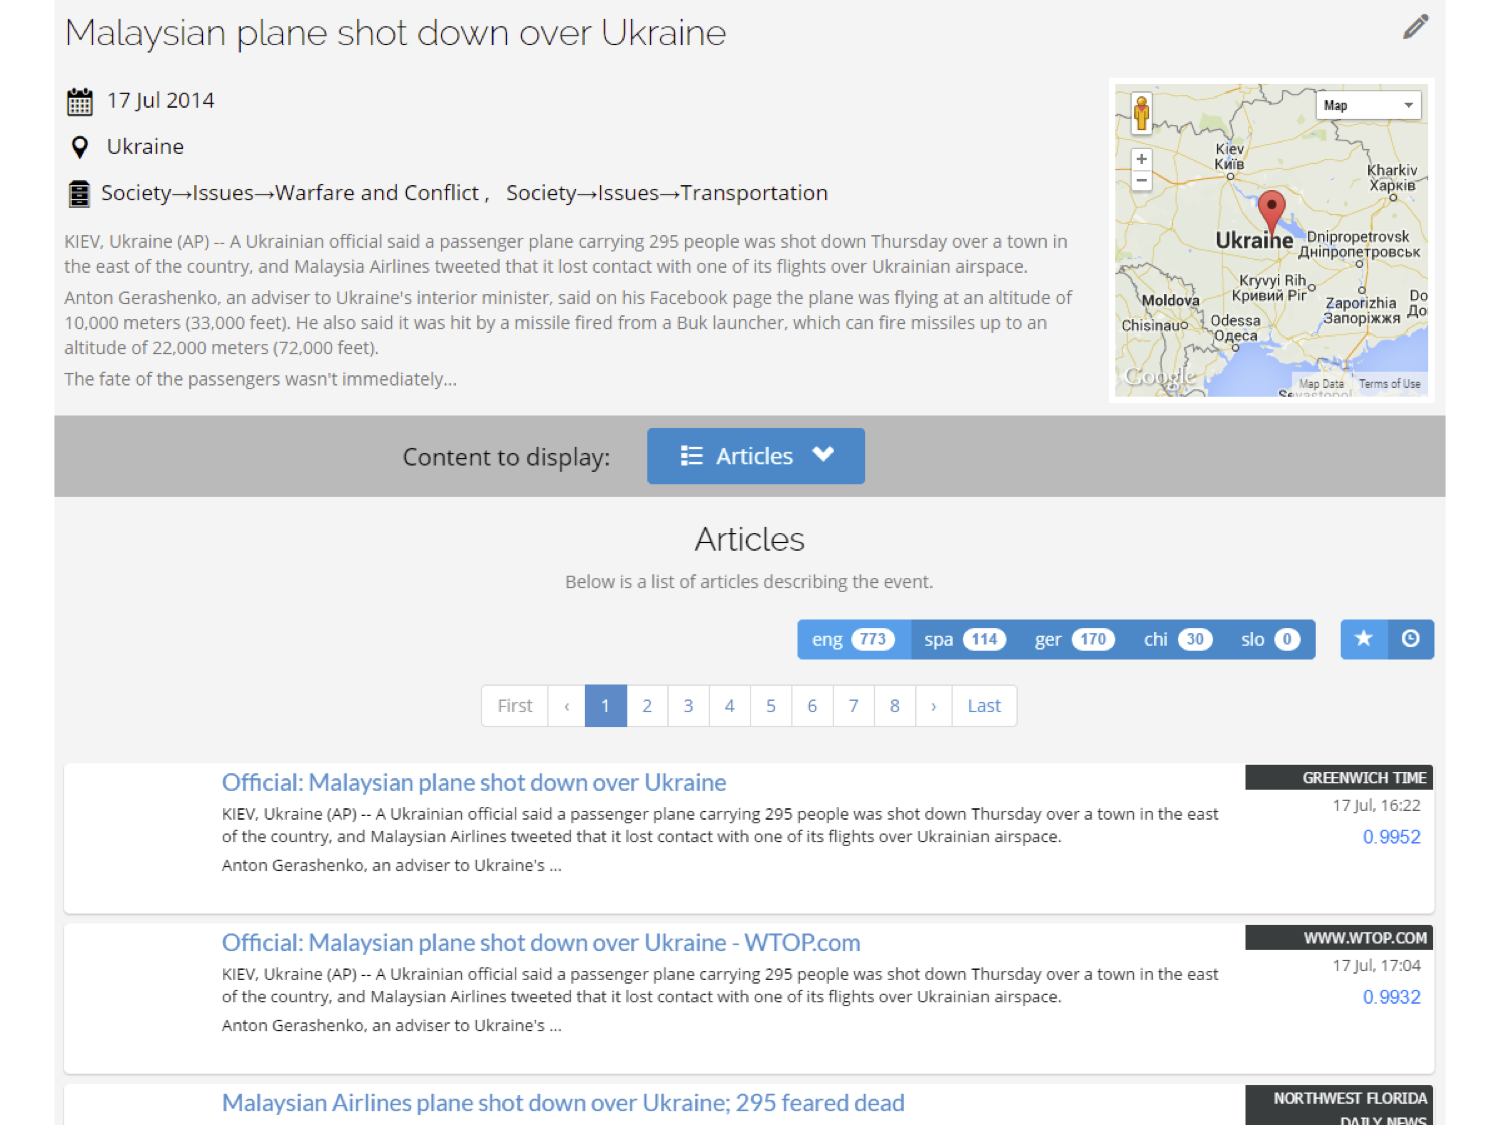
\includegraphics[width=0.75\textwidth]{events2.png}
\caption{\label{fig:event2} Events are represented by collections of articles about an event, in this case the Malaysian airliner which was shot down over the Ukraine.}
\end{figure}

As input we consider a stream of articles in different languages and a list of events. Our goal is to assign articles to their corresponding events. A priori we do not know the coverage of the articles, that is not all the events may be covered and we do not know that all the articles necessarily fit into one of the events. The task is divided into two parts: detecting events within each language and then linking events across languages. In this paper we address the second step.

As input we consider a high volume of articles in different languages. By using a language detector the stream is split into separate monolingual streams. Within each monolingual stream, an online clustering approach is employed, where tracked clusters correspond to our definition of events - this is based on the Event Registry system \shortcite{Leban2014W,Leban2014I}. Our main goal in this paper is to connect such clusters (representations of events) across languages, that is detect that a set of articles in language $A$ reports on the same event as a set of articles in language $B$.

Our approach to linking clusters across languages combines two ingredients: a cross-lingual document similarity measure, which can be interpreted as a language independent topic model, and semantic annotation of documents, which enables an alternative way to comparing documents.

The first approach represents a continuation of previous work \shortcite{nips,sikdd,nips2,iti} where we explored representations of documents which were valid over multiple languages.  The representations could be interpreted as multi-lingual topics, which were then used as proxies to compute cross-lingual similarities between documents. To learn the representations, we use Wikipedia as a training corpus. Significantly, we do not only consider the major or \emph{hub} languages such as English, German, French, etc. which have significant overlap in article coverage, but also smaller languages (in terms of number of Wikipedia articles) such as Slovenian and Hindi, which may have a negligible overlap in article coverage. We can then define a similarity between any two articles regardless of language,  which allows us to cluster the articles according to topic. The underlying assumption being that articles describing the same event are similar  and will therefore be put into the same cluster.

Based on the similarity function we propose a novel algorithm for linking events/clusters across languages. The approach is based on learning a classification model from labelled data based on several sets of features. In addition to these features, cross-lingual similarity is also used to quickly identify a small list of potential linking candidates for each cluster.
This greatly increases the scalability of the system.

%As input we consider a stream of articles in different languages and a list of events. Our goal is to assign articles to their corresponding events. A priori we do not know the coverage of the articles, that is not all the events may be covered and we do not know that all the articles necessarily fit into one of the events.  To achieve our goal, we divide the task into two parts: clustering the articles according to topic (regardless of language) and matching the clusters to events.
%
%To cluster the articles, rather than rely on machine translations, we adopt well-established monolingual text mining tools to the multilingual setting. This represents the continuation of previous work \shortcite{nips,sikdd,nips2,iti} where we explored representations of documents which were valid over multiple languages.  The representations could be interpreted as multi-lingual topics, which were then used as proxies to compute cross-lingual similarities between documents. To learn the representations, we use Wikipedia as a training corpus. Significantly, we do not only consider the major or \emph{hub} languages such as English, German, French, etc. which have significant overlap in article coverage, but also smaller languages (in terms of number of Wikipedia articles) such as Slovenian and Hindi, which may have a negligible overlap in article coverage. We can then define a similarity between any two articles regardless of language,  which allows us to cluster the articles according to topic. The underlying assumption being that articles describing the same event are similar  and will therefore be put into the same cluster.
%
%The second step is to match our computed clusters to events. Since our similarity measure and clustering
%may not be perfect, we need to find the ``best" correspondence between clusters and events. In this paper, we test several different algorithms for both steps for performance in an integrated system. In particular, we test our approach within an online system for detection of world events, called Event Registry \shortcite{Leban2014W,Leban2014I}. Event Registry is a repository of events, where events are automatically identified by analyzing news articles.

%
%Event Registry works by collecting and analyzing news articles that are published by news outlets in different languages all over the world. Collected articles are first semantically annotated by identifying in them mentions of relevant concepts -- either entities or important keywords. The disambiguation and entity linking of the concepts is done using Wikipedia as the main knowledge base.
%   The key step in Event Registry is then to apply an online clustering algorithm on the articles in order to identify groups of articles that are discussing the same event.
%
%   Within this system, we test our multilingual similarity measures as well as our algorithms for matching clusters across languages.  The result is that we can test total performance in a multilingual, real-world setting.

The paper is organized as follows: we first provide an overview of the system as a whole (Section ~\ref{sec:pipeline}), followed by details on each of the two steps described above. We first introduce several approaches for measuring cross-lingual similarity (Section~\ref{sec:crosslingual}) and then the algorithms for matching clusters in different languages (Section~\ref{sec:linking}).  To improve readability, we describe relevant related work for each module in its corresponding Section. Finally, we present and interpret the experimental results, give conclusions and describe promising future directions.


\section{Pipeline}\label{sec:pipeline}

\begin{figure}[tb]
\centering
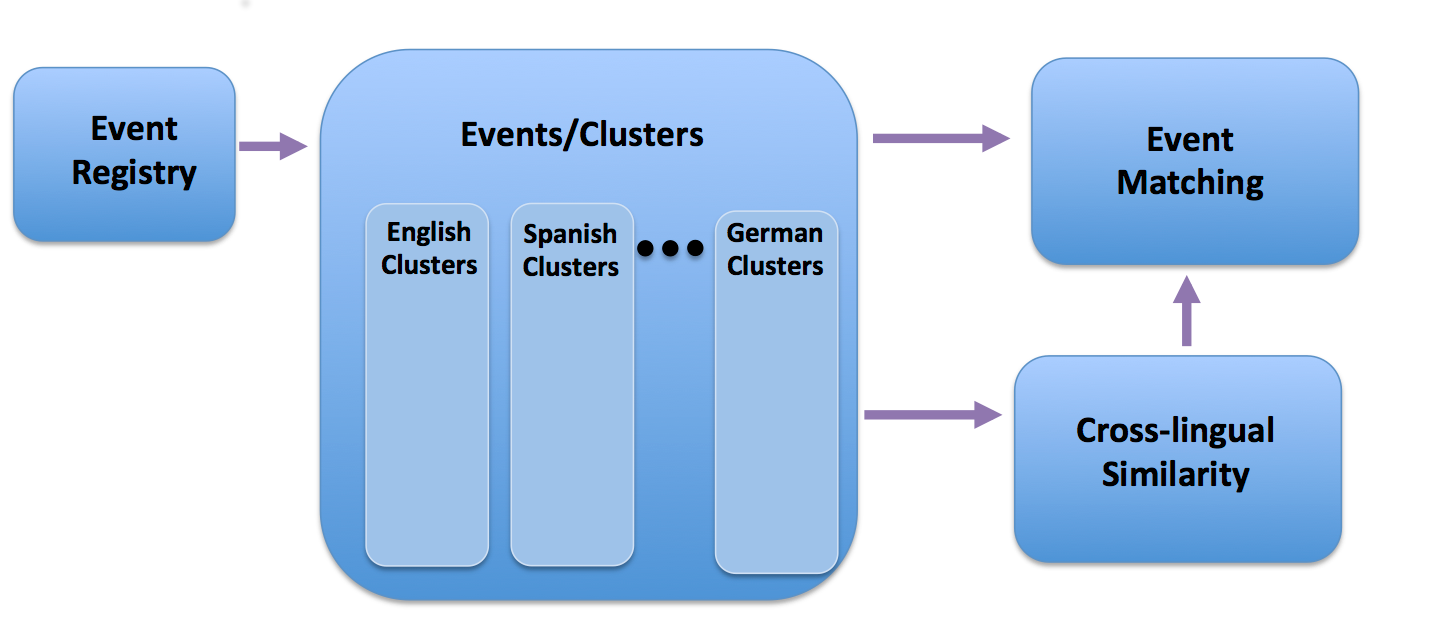
\includegraphics[width=0.75\textwidth]{pipeline1}
\caption{\label{fig:pipeline} Our pipeline - from the Event Registry we obtain a stream of multi-lingual documents and monolingual clusters. Our contribution is shown on the right, where using cross-lingual similarity, we link the clusters across languages which correspond to the same event.}
\end{figure}

We base our techniques of cross-lingual event linking on an online system for detection of world events, called Event Registry \shortcite{Leban2014W,Leban2014I}. Event Registry is a repository of events, where events are automatically identified by analyzing news articles.  Event Registry works by collecting and analyzing news articles that are published by news outlets in different languages all over the world. Collected articles are first semantically annotated by identifying in them mentions of relevant concepts -- either entities or important keywords. The disambiguated and entity linking of the concepts is done using Wikipedia as the main knowledge base. An online clustering algorithm is then applied on the articles in order to identify groups of articles that are discussing the same event. For each new article, the clustering algorithm determines if the article should be assigned to some existing cluster or into a new cluster. The underlying assumption is that articles that are describing the same event are similar enough and will therefore be put into the same cluster.

The processing is done independently for each language and the output is a clustering of articles in each language, with each cluster ideally representing an event, which are defined by topically, geographically and temporally. The goal of this paper is present approaches to  connecting the clusters/events across languages.

Our approach is based on first defining a similarity function between articles in different languages (Section~\ref{sec:crosslingual}) and then we present several efficient approaches to linking the clusters based on features (Section~\ref{sec:linking}). The pipeline is shown in Figure~\ref{fig:pipeline} First, however we describe the pre-processing on the input articles which we then take as input.


The system is designed to handle streams and so we describe how a document which enters the stream is processed. The sequence of operations is shown in  Figure~\ref{fig:erpipeline}.  A new document is first tokenized, stop words are removed and words are stemmed.
 What remains is represented in a vector-space model and normalized using $TF-IDF$ (see Section~\ref{sec:tfidf} for the definition). Since each article is tagged with its language, cosine similiarity  is used to find the modst similar existing cluster, by comparing it to the centroid vector of each cluster. A selected threshold is used to determine if the article is not similar to any existing clusters (0.4 was used in our experiments).  The article is then assigned to the corresponding cluster, otherwise a new cluster is created, initially containing only the single article.


Since articles about an event are commonly written only for a short period of time, we remove clusters once the oldest article in the cluster becomes more than 4 days old. This housekeeping mechanism prevents the clustering from becoming slow and also ensures that articles are not assigned to obsolete clusters.

The clusters, we consider must have a sufficient number of articles (which is a language dependent paramater). This is to ensure that we consider events. Once an event is identified(i.e. a cluster of sufficient size), a new unique ID is assigned to it and the main information about the event is then automatically extracted by analyzing the articles assigned to it. The extracted information includes properties such as the date of the event, the location, who is involved in it, what the event is about, etc.

 Further details about the system can be found in \cite{}.

\begin{figure}[tbp]
\centering
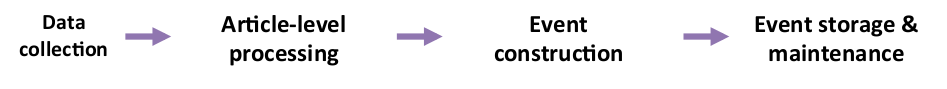
\includegraphics[width=\textwidth]{ev_pipeline}
\caption{\label{fig:erpipeline}  The Event Registry pipeline, after obtaining the raw stream of multi-lingual news articles, it first cleans and processes articles individually. It then aggregates and clusters the articles into similar events (within each language) and finally provides an interface allowing us to query for articles.}
\end{figure}

\begin{comment}
In short, the article clustering works as follows (details are available in \cite{}). First we create a new document by joining the title and the body of the article. We then tokenize the document, remove the stop words and stem the words. The remaining words are represented as a vector in the vector-space model. Each value in the vector is additionally normalized using TF-IDF. After normalization, we use the vector to find the most similar existing cluster. To be able to compare the vector with a cluster we first need a vector representation for each of the clusters. This is done by computing a centroid vector of the cluster by simply averaging the vectors of the articles in the cluster. By computing the cosine similarity of the article vector with each of the centroid vectors we then find the cluster with the highest similarity. If the highest similarity is above the selected threshold (we used 0.4 in our experiments),


In order to treat the cluster as describing an event in Event Registry,

The clustering of articles is done for each language separately -- English articles are, for example, clustered separately from Spanish articles. When events are identified, they will therefore be identified from clusters in each language separately. As a result, the same event will be represented in Event Registry with two or more event IDs, and each event will only contain coverage in a single language. To avoid this problem we want to exploit the available information about the similarity of the articles in a cluster with articles in other languages. Using this information we hope to be able to connect clusters in different languages and represent them using a single event ID.
\end{comment}
%Event registry $\Rightarrow$ Monolingual events $\Rightarrow$ features (semantic + CCA) $\Rightarrow$ linked events (crosslingual)


\section{Cross-lingual Document Similarity}
\label{sec:crosslingual}
Document similarity is an important component in techniques from text mining and natural language processing. Many techniques use the similarity as a black box, i.e., a kernel in Support Vector Machines. Comparison of documents (or other types of text snippets) is a well studied problem \todo{some references to prove that}. In this section we define document similarity in a cross-lingual setting, where the similarity function receives documents in different languages. We conclude the section by an introduction of \todo{two datasets} which we used in this paper to learn cross-lingual similarity functions.

\subsection{Related work}

In this section we will relate the method we use to other alternatives in the literature. We will first state some requirements for our system, which motivate our choice of focusing on a particular subset of approaches in the rest of the paper.

The goal is to build a system that monitors global media and analyzes how events are being reported on. In our approach this boils down to two steps: tracking events separately in each language (based on language detection and an online clustering approach) and then connecting them. The pipeline needs to process millions of articles per day and perform billions of similarity computations each day. The system should support as many languages as possible. We focus on implementations that run on a single shared memory machine, as opposed to clusters of machines. This severely simplifies the software implementation and the system maintenance.
To summarize, the following properties are desireable:
\begin{itemize}
\item \textbf{training} - The training (building corss-lingual models) should scale to many languages and should be robust to the quality of training resources. The system should be able to take advantage of comparable corpus (as opposed to parallel translation based corpora), with missing data. Supporting a new language should be simple.
\item \textbf{operation efficiency} - The similarity computation should be fast - the system needs to handle billions of similarity computations per day.
\item \textbf{operation cost} - The system should run on a strong shared machine server and not rely on paid services.
\item \textbf{implementation} - The system is simple to implement, with few parameters to tune.
\end{itemize}
We believe that a cross-lingual similarity component that meets such requirements is very desirable in a commercial setting, where several different costs have to be taken into consideration.

There are three main families of approaches to cross-lingual similarity.
\begin{itemize}
\item \textbf{translation} - The most obvious way to compare documents written in different languages is to use machine translation and perform monolingual similarity. One can use free tools such as Moses \shortcite{moses} or translation services, such as Google Translate\footnote{https://translate.google.com/}. There are two issues with such approaches: they solve a harder problem than needs to be solved and they are less robust to training resource quality - large sets of translated sentences are typically needed. Training Moses for languages with scarce linguistic resources is thus problematic. The issue with using online services such as Google Translate is that the APIs are limited and not free. The operation efficiency and cost requirements make translation based approaches less suited for our system.
\item \textbf{probabilistic topic models} -  There exist many variants to modelling documents in a language independent way by using probabilistic graphical models. The models include:  Joint Probabilistic Latent Semantic Analysis (JPLSA) \shortcite{platt2010translingual}, Coupled Probabilistic LSA (CPLSA) \cite{platt2010translingual}, Probabilistic Cross-Lingual LSA (PCLLSA)\cite{PCL_LSA} and Polylingual Topic Models (PLTM) \shortcite{polyLDA} which is a Bayesian version of PCLLSA. The methods (except for CPLSA) describe the multilingual document collections as samples from generative probabilistic models, with variations on the assumptions on the model structure. The topics represent latent variables that are used to generate observed variables (words), a process specific to each language. The parameter estimation is posed as an inference problem which is typically intractable and one usually solves it using approximate techniques. Most variants of solutions are based on Gibbs sampling or Variational Inference, which are not trivial to implement and may require an experienced practitioner to apply. Furthermore, representing a new document as a mixture of topics is another potentially hard inference problem which needs to be solved.
\item \textbf{classification problem related} - In approaches such as \cite{cotrain} and \shortcite{svm2k} the authors find linear embeddings of the data that support good classification results, based on a given classification problem training data. We do not consider this family of approaches, since for general language pairs classifier training sets may not be available.
\item \textbf{matrix factorization} - Non-negative matrix factorization based \cite{nonnegfactor_lsi}, Cross-Lingual Latent Semantic Indexing CLLSI\shortcite{cl_lsi}, Canonical Correlation Analysis (CCA) \cite{Hotelling}, Oriented Principal Component Analysis \cite{platt2010translingual}. The quadratic time and space dependency of the OPCA method makes it impractical for large scale purposes. In addition, OPCA forces the vocabulary sizes for all languages to be the same, which is less intuitive. For our setting, the method in \cite{nonnegfactor_lsi} has a prohibitively high computational cost when building models (it uses dense matrices of dimensions that is the product of training set size and vocabulary size). Our proposed approach combines CCA and CLLSI, which will be presented in more detail.

\end{itemize}

Based on the discussion above, we chose to focus on methods based on vector space models and linear embeddings. We propose a method that is more efficient than popular alternatives (a clustering based approach and latent semantic indexing), but is still simple to optimize and use.

\subsection{Problem definition}
\label{sec:tfidf}
\textbf{Document representation.}

Standard vector space model \cite{Salton88term-weightingapproaches} represents documents as vectors, where each term corresponds to word or phrase in a fixed vocabulary. More formally, document $d$ is represented by a vector $x \in \RR^n$, where $n$ corresponds to the size of the vocabulary, and vector elements $x_k$ correspond to the number of times term $k$ occurred in the document, also called \emph{term frequency} or $TF_k(d)$.

We also used a term re-weighting scheme that adjusts for the fact that some words occur more frequently in general. A term weight should correspond to the importance of the term for the given corpus. The common weighting scheme is called \emph{Term Frequency Inverse Document Frequency} ($TFIDF$) weighting. An \emph{Inverse Document Frequency} ($IDF$) weight for the dictionary term $k$ is defined as $\log\left( \frac{N}{DF_k} \right)$, where $DF_k$ is the number of documents in the corpus which contain term $k$.  A document $TFIDF$ vector is its original vector multiplied element-wise by the weights.

The $TFIDF$ weighted vector space model document representation corresponds to a map $\phi : \text{text} \rightarrow \RR^n$ defined by:
$$\phi(d)_k = {TF}_k(d) \log\left( \frac{N}{{DF}_k}\right).$$

\textbf {Mono-lingual similarity.}
A common way of computing similarity between documents is \emph{cosine similarity},
$$sim(d_1, d_2) = \frac{\langle \phi(d_1), \phi(d_2)\rangle}{\|\phi(d_1)\| \|\phi(d_2)\|},$$
where $\langle \cdot,\cdot \rangle$ and $\|\cdot\|$ are standard inner product and Euclidean norm. Cosine similarity, and other related approaches, assumes that the similarity is reflected in the overlap of words, and as such works only when the documents $d_1$ and $d_2$ are written in the same language.

\textbf {Cross-lingual similarity.}
Processing a multilingual dataset results in several vector spaces with varying dimensionality, one for each language. The dimensionality of the vector space corresponding to the $i$-th language is denoted by $n_i$ and and the vector space model mapping is denoted by $\phi_i : \text{text} \rightarrow \RR^{n_i}$.
The similarity between documents in language $i$ and language $j$ is defined as a bilinear operator represented as a matrix $S_{i,j} \in \RR^{n_i \times n_j}$:
$$sim_{i,j}(d_1, d_2) = \frac{ \langle \phi_i (d_1), S_{i,j} \phi_j (d_2) \rangle }{\|\phi_i(d_1)\| \|\phi_j(d_2)\|},$$
where $d_1$ and $d_2$ are documents written in the $i$-th and $j$-th language respectively. If the the maximal singular value of $S_{i,j}$ is bounded by $1$, then the similarity scores will lie on the interval $[-1, 1]$. In section \ref{sec:models} we will describe some approaches to computing $S_{i,j}$ given training data.

\section{Multilingual Latent Factor Models}\label{sec:models}
In this section, we describe several approaches to computing multilingual simliarities described in the previous section. We present three approaches
\begin{enumerate}
\item  a simple approach based on $k$-means clustering
\item  a standard approach based on singular value decomposition
\item a new method that is applicable in more general settings.
\end{enumerate}
 We concentrate on approaches that are based on linear maps rather than alternatives, such as machine translation and probabilistic models. Applicability of machine translation relies
on the availability of training resources (strongly aligned translation corpora), which are not available for many world languages, but there exist comparable corpora. Probabilistic
methods \todo{provide reasons for not using them: e.g. difficulty with parameter estimation, maybe just say future work?}.

For completeness we will also present the method of Canonical Correlation Analysis, since it is related to our proposed method.

\subsection{Notation}

The cross-lingual similarity models presented in this paper are based on comparable corpora. That is, a corpus of documents in multiple languages, with alignment between documents that are of the same topic, or even a rough translation of each other. Wikipedia is an example of a comparable corpus, where a specific entry can be described in multiple languages (e.g. "Berlin" is currently described in 222 languages). News articles represent another example, where the same event can be described by newspapers in several languages.

More formally, \emph{multilingual document} $d = (u_1,\ldots u_m)$ is a tuple of $m$ documents on the same topic (comparable), where $u_i$ is the document written in language $i$. Note that individual document $u_i$ can be an empty document (missing resource) and each $d$ must contain at least two nonempty documents. A comparable corpus $D = {d_1, \ldots, d_N}$ is a collection of multilingual documents. By using the vector space model we can represent $D$ as a set of $m$ matrices $X_1,\ldots,X_m$, where $X_i \in \RR^{n_i \times N}$ is the matrix corresponding to the language $i$ and $n_i$ is the vocabulary size of language $i$. Furthermore, let $X_i^{\ell}$ denote the $\ell$-th column of matrix $X_i$ and the matrices respect the document alignment - the vector $X_i^\ell$ corresponds to the TFIDF vector of the $i$-th component of multilingual document $d_\ell$. We use $N$ to denote the total row dimension of $X$, i.e. $N:= \sum_{i=1}^m n_i$.


\subsection{$k$-means}

The $k$-means algorithm is perhaps the most well-known and widely-used clustering algorithm. In order to apply the algorithm, we first merge all the term-document matrices into a single matrix $X$ by stacking the individual term-document matrices:
$$X := \begin{bmatrix}X_1^T ,X_2^T, \cdots, X_m^T \end{bmatrix}^T,$$
such that the columns respect the alignment of the documents (here MATLAB notation for concatenating matrices is used). Therefore, each document  is represented by a long vector indexed by the terms in all languages.

We then run the $k$-means algorithm \cite{kmeans} and obtain a centroid matrix $C \in \RR^{N \times k}$, where the $k$ columns represent centroid vectors. The centroid matrix can be split vertically into $m$ blocks: $$C = [C_1^T \cdots C_m^T]^T,$$ according to the number of dimensions of each language, i.e. $C_i \in \RR^{n_i \times k}$.

Each matrix $C_i$ represents a vector space basis and can be used to map points in $\RR^{n_i}$ into a $k$-dimensional space, where the coordinates of a vector $x \in \RR^{n_i}$ are expressed as: $$(C_i^T C_i)^{-1} C_i^T x_i.$$

The resulting matrix (when appropriately scaled to have unit norm) for similarity computation between language $i$ and language $j$ is defined as (see the reasoning below):
$$C_i(C_i^T C_i)^{-1} (C_j^T C_j)^{-1} C_j.$$

The matrix is a result of mapping documents in a language independent space using pseudo-inverses of the centroid matrices $P_i = (C_i^T C_i)^{-1} C_i$ and then comparing them using the standard inner product, which results in the matrix $P_i^T P_j$. For the sake of presentation, we assumed that the centroid vectors are linearly independent (an independent subspace could be obtained using an additional Gram-Schmidt step on the matrix $C$, if this was not the case).

\subsection{Cross-Lingual Latent Semantic Indexing}

The next method is Cross-Lingual Latent Semantic Indexing (CL-LSI)\cite{cl_lsi} which is a variant of LSI~\shortcite{lsi} for more than one language. The method is based on computing a truncated singular value decomposition of $X \approx U S V^T$. Since the matrix can be large we can use an iterative method like the Lanczos~\cite{golub} algorithm with reorthogonalization to find the left singular vectors (columns of $U$) corresponding to the largest singular values. It turns out that the Lanczos method converges slowly as the gap between the leading singular values is small. Moreover, the Lanczos method is hard to parallelize. Instead we use a randomized version of the singular value decomposition (SVD) described in \shortcite{tropp} that can be viewed as a block Lanczos method. That enables us to use parallelization and speeds up the computation considerably.

The cross-lingual similarity functions are based on a rank-$k$ truncated SVD: $X \approx U \Sigma V^T,$ where $U \in \RR^{N \times k}$ are basis vectors of interest and $\Sigma \in \RR^{k \times k}$ is truncated diagonal matrix of singular eigenvalues.

An aligned basis is obtained by first splitting $U$ vertically according to the number of dimensions of each language: $U = [U_1^T \cdots U_m^T]^T$. Then, the same as with $k$-means clustering, we compute the pseudoinverses $P_i = (U_i^T U_i)^{-1} U_i^T$. The matrices $P_i$ are used to change the basis from the standard basis in $\RR^{n_i}$ to the basis of columns of $U_i$.

The numerical implementation of the least squares is done by QR algorithm, by computing factorizing $U_i = Q R$, where $Q^TQ = I$ and $R$ is triangular matrix. $P_i$ is then obtained by solving $R P_i = Q$.


\subsection{Canonical Correlation Analysis}\label{sec:CCA}
 The final approach is a statistical technique to analyze data from two sources - after which we will describe our main contribution to computing cross-lingual similarities.

 Canonical Correlation Analysis (CCA)~\cite{Hotelling} is a dimensionality reduction technique similar to Principal Component Analysis (PCA)~\cite{Pearson1901On}, with an additional assumption that the data consists of feature vectors that arose from two sources (two views) that share some information (examples: bilingual document collection~\shortcite{mrpqr}, collection of images and captions~\shortcite{Hardoon_usingimage}). Instead of looking for linear combinations of features that maximize the variance (PCA) we look for a linear combination of feature vectors from the first view and a linear combination for the second view, that are maximally correlated.

Interpreting the columns of $X_i$ as observation vectors sampled from an underlying distribution $\mathcal{X}_i \in \RR^{n_i}$, the idea is to find two weight vectors $w_i \in \RR^{n_i}$ and $w_j \in \RR^{n_j}$ so that the random variables $w_i^T \cdot \mathcal{X}_i$ and $w_j^T \cdot \mathcal{X}_j$ are maximally correlated ($w_i$ and $w_j$ are used to map the random vectors to random variables, by computing weighted sums of vector components). Let $\rho(x,y)$ denote the sample based correlation coefficient between two vectors of observations $x$ and $y$. By using the sample matrix notation $X_i$ and $X_j$ (assuming no data is missing for clearer presentation) this problem can be formulated as the following optimization problem:
\begin{equation*}
\begin{aligned}
& \underset{w_i \in \RR^{n_i}, w_j \in \RR^{n_j}}{\text{maximize}}
& & \rho(w_i^T X_i , w_j^T X_j) = \frac{w_i^T C_{i,j} w_j}{\sqrt{w_i^T C_{i,i} w_i} \sqrt{w_j^T C_{j,j} w_j}},
\end{aligned}
\end{equation*}
where $C_{i,i}$ and $C_{j,j}$ are empirical estimates of variances of $\mathcal{X}_i$ and $\mathcal{X}_j$ respectively and $C_{i,j}$ is an estimate for the covariance matrix. Assuming that the observation vectors are centered (only for the purposes of presentation), the matrices are computed in the following way: $C_{i,j} = \frac{1}{n-1}X_i X_j^T$, and similarly for $C_{i,i}$ and $C_{j,j}$.
The optimization problem can be reduced to an eigenvalue problem and includes inverting the variance matrices $C_{i,i}$ and $C_{j,j}$. If the matrices are not invertible, one can use a regularization technique by replacing $C_{i,i}$ with $(1- \kappa)C_{i,i} + \kappa I$, where $\kappa \in [0,1]$ is the regularization coefficient and $I$ is the identity matrix (the same can be applied to $C_{j,j}$.
A single canonical variable is usually inadequate in representing the original random vector and typically one looks for $k$ projection pairs $(w_i^1, w_j^1),\ldots,(w_i^k, w_j^k)$, so that $(w_i^{u})^T \mathcal{X}_i$ and $(w_j^{u})^T \mathcal{X}_j$ are highly correlated and $(w_i^{u})^T \mathcal{X}_i$ is uncorrelated with $(w_i^{v})^T \mathcal{X}_i$  for $u \neq v$ and analogously for $w_j^u$ vectors.

Note that the method in its original form is only applicable to two languages where an aligned set of observations is available.

\subsection{Hub languages}

In this section, we describe an extension to CCA, but is more applicable to a large number of languages. The main difficulty with applying the
LSI and $k$-means approaches lies in the fact, that when one considers a large number of languages, for example, the top 100 Wikipedia languages (ranked by number of articles), the set of completely
aligned documents is often small or empty. Even if only two languages are considered, the set of aligned documents can be small (for example, Piedmontese and Hindi
Wikipedias had no interlanguage links). In Wikipedia, we observed that even though the training resources are scarce between certain language pairs, there often exists indirect training data
through what we refer to as a hub language.

A \emph{hub language} is a language with a high proportion of non-empty documents in $D = \left\{d_1,..., d_{\ell}\right\}$. The prototypical  exampling  in the case of Wikipedia is English. We use the following notation to define subsets of the multilingual comparable corpus: let $a(i,j)$ denote the index set of all multilingual documents with non-missing data for the $i$-th and $j$-th language:  $$a(i,j) = \left\{k~ |~ d_k = (u_1,...,u_m), u_i \neq \emptyset, u_j \neq \emptyset \right\},$$ and let $a(i)$ denote the index set of all multilingual documents with non missing data for the $i$-th language.

We now describe a two step approach to building a cross-lingual similarity matrix. The first part is related to LSI and reduces the dimensionality of the data. The second step refines the linear mappings and optimizes linear dependence between data.

The first step in our method is to project $X_1, \ldots, X_m$ to lower dimensional spaces without destroying the cross-lingual structure. Treating the nonzero columns of $X_i$ as observation vectors sampled from an underlying distribution $\mathcal{X}_i \in V_i = \RR^{n_i}$, we can analyze the empirical cross-covariance matrices:
$$C_{i,j} = \frac{1}{|a(i,j)|-1 }\sum_{\ell \in a(i,j)} (X_i^{\ell} - c_i)\cdot (X_j^{\ell} - c_j)^T,$$
 where $c_i = \frac{1}{a_i} \sum_{\ell \in a(i)}X_i^{\ell}$. By finding low rank approximations of $C_{i,j}$ we can identify the subspaces of $V_i$ and $V_j$ that are relevant for extracting linear patterns between $\mathcal{X}_i$ and $\mathcal{X}_j$. Let $X_1$ represent the hub language corpus matrix. The LSI approach to finding the subspaces is to perform the singular value decomposition on the full $N \times N$ covariance matrix composed of blocks $C_{i,j}$. If $|a(i,j)|$ is small for many language pairs (as it is in the case of Wikipedia), then many empirical estimates $C_{i,j}$ are unreliable, which can result in overfitting. For this reason we perform the truncated singular value decomposition on the matrix $C = [C_{1,2}  \cdots  C_{1,m}] \approx U S V^T$, where where $U \in \RR^{n_1 \times k}, S \in \RR^{k \times k}, V \in \RR^{(\sum_{i=2}^m n_i) \times k}$. We split the matrix $V$ vertically in blocks with $n_2, \ldots, n_m$ rows: $V = [V_2^T  \cdots  V_m^T]^T$. Note that columns of $U$ are orthogonal but columns in each $V_i$ are not (columns of V are orthogonal). Let $V_1 := U$. We proceed by reducing the dimensionality of each $X_i$ by setting: $Y_i = V_i^T \cdot X_i$, where $Y_i \in \RR^{k\times N}$. To summarize, the first step reduces the dimensionality of the data and is based on CL-LSI, but optimizes only the hub-language related cross-covariance blocks.

The second step involves solving a generalized version of canonical correlation analysis on the matrices $Y_i$ in order to find the mappings $P_i$. The approach is based on the sum of squares of correlations formulation by Kettenring \cite{Kettenring}, where we consider only correlations between pairs $(Y_1, Y_i), i >1$ due to the hub language problem characteristic.
We will present the original unconstrained optimization problem, then a constrained formulation based on the hub language problem characteristic. Then we will simplify the constraints and reformulate
the problem as an eigenvalue problem by using the method of Lagrange multipliers.

The original sum of squared correlation is formulated as an unconstrained problem:
\begin{equation*}
  \begin{aligned}
    & \underset{w_i \in \RR^{k}}{\text{maximize}}
    & & \sum_{i < j}^m  \rho(w_i^T Y_i, w_j^T Y_j)^2.
\end{aligned}
\end{equation*}
We solve a similar problem by restricting $i=1$ and omit optimizing over non-hub language pairs.
Let $D_{i,i} \in \RR^{k \times k}$ denote the empirical covariance of $\mathcal{Y}_i$ and $D_{i,j}$ denote the empirical cross-covariance computed based on $\mathcal{Y}_i$ and $\mathcal{Y}_j$. We solve the following constrained (unit variance constraints) optimization problem:
\begin{equation}\label{squaredCorHubOriginal}
  \begin{aligned}
    & \underset{w_i \in \RR^{k}}{\text{maximize}}
    & & \sum_{i = 2}^m  \left(w_1^T D_{1,i} w_i \right)^2
    & \text{subject to}
    & & w_i^T D_{i,i} w_i = 1, \quad\forall i = 1,\ldots, m.
\end{aligned}
\end{equation}
The constraints $w_i^T D_{i,i} w_i$ can be simplified by using the Cholesky decomposition $D_{i,i} = K_i^T \cdot K_i$ and substitution: $y_i := K_i w_i$. By inverting the $K_i$ matrices and defining  $G_i := K_1^{-T} D_{1,i} K_i^{-1}$, the problem can be reformulated:
\begin{equation}\label{squaredCorHub}
  \begin{aligned}
    & \underset{y_i \in \RR^{k}}{\text{maximize}}
    & & \sum_{i = 2}^m  \left(y_1^T G_{i} y_i \right)^2
    & \text{subject to}
    & & y_i^T y_i = 1, \quad\forall i = 1,\ldots, m.
\end{aligned}
\end{equation}
A necessary condition for optimality is that the derivatives of the Lagrangian vanish. The Lagrangian of (\ref{squaredCorHub}) is expressed as:
$$  L(y_1, \ldots, y_m, \lambda_1, \ldots, \lambda_m) = \sum_{i = 2}^m  \left(y_1^T G_{i} y_i \right)^2 + \sum_{i=1}^m \lambda_i \left(y_i^T y_i - 1\right).$$
Stationarity conditions give us:
\begin{equation}\label{dLdx1}
 \frac{\partial}{\partial x_1} L = 0 \Rightarrow \sum_{i = 2}^m  \left(y_1^T G_{i} y_i \right) G_i y_i + \lambda_1 y_1,
\end{equation}
\begin{equation}\label{dLdxi}
\frac{\partial}{\partial x_i} L = 0 \Rightarrow \left(y_1^T G_{i} y_i \right) G_{i}^T y_1 + \lambda_i y_i = 0,~i > 1.
\end{equation}
Multiplying the equations (\ref{dLdxi}) with $y_i^T$ and applying the constraints, we can eliminate $\lambda_i$ which gives us:
\begin{equation}\label{eqy1yi}
G_{i}^T y_1 = \left(y_1^T G_{i} y_i \right) y_i,~i > 1.
\end{equation}
Plugging this into (\ref{dLdx1}), we obtain an eigenvalue problem:
$$\left( \sum_{i = 2}^m G_i G_{i}^T \right) y_1 + \lambda_1 y_1 = 0.$$
The eigenvectors of $\left( \sum_{i = 2}^m G_i G_{i}^T \right)$ solve the problem for the first language. The solutions for $y_i$ are obtained from (\ref{eqy1yi}): $y_i := \frac{G_{i}^T y_1}{\| G_{i}^T y_1 \|}$.
Note that the solution (\ref{squaredCorHubOriginal}) to can be recovered by: $w_i := K_i^{-1} y_i$. The linear transformation of the $w$ variables are thus expressed as:
$$ Y_1 := \text{eigenvectors of} \sum_{i = 2}^m G_i G_{i}^T, $$
$$ W_1 = K_1^{-1} Y_1 $$
$$ W_i = K_i^{-1} G_{i}^T Y_1 N,$$
where $N$ is a diagonal matrix that normalizes $G_{i}^T Y_1$, with $N(j,j) := \frac{1}{\|G(_{i} Y_1(:,j)\|}$.

 The technique is related to the Generalization of Canonical Correlation Analysis (GCCA) by Carroll \citeyear{Carroll}, where an unknown group configuration variable is defined and objective is to maximize the sum of squared correlation between the group variable and the others. The problem can be reformulated as an eigenvalue problem. The difference lies in the fact that we set the unknown group configuration variable as the hub language, which simplifies the solution. The complexity of our method is $O(k^3)$, whereas solving the GCCA method scales as $O(N^3)$ where $N$ is the number of samples (see \cite{gifi}). Another issue with GCCA is that it cannot be directly applied to the case of missing documents.

To summarize, we first reduced the dimensionality of our data to $k$-dimensional features and then found a new representation (via linear transformation) that maximizes directions of linear dependence between the languages. The final projections that enable mappings to a common space are defined as: $P_i(x) = W_i^T V_i^T x.$

(figure?)


\section{Cross-lingual Event Linking}

The main application on which we test the above similarity is cross-lingual event linking. In online media streams -- particularly new articles -- there is often duplication of reporting, different viewpoints or opinions, all centering around a single event. Same events are covered by many articles and the question we address is how to find all the articles in different languages that are describing a single event. We base our evaluation on an online system for detection of world events, called Event Registry. We do not address the problem of detection of events in this paper but rather consider the problem that given a series of events, how may we best ``tag" or match articles in different languages to these events. The events are represented by clusters of articles and so ultimately our problem reduces to find suitable matchings between clusters with articles in different languages.

\subsection{Problem definition}

The problem of cross-lingual event linking is to identify the clusters describing the same events. Each article $a_i$ is written in a language $l$, where $\ell \in L = \{\ell_1,\ell_2,...,\ell_k\}$. For each language $\ell$, we generate and maintain a set of language-specific clusters $C_l$. That is, all articles are in language $l$. For any cluster $c_i \in C_{\ell_a}$, we would like to identify clusters $c_j \in C_{\ell_b}$ (where $\ell_a \neq \ell_b$) that describe the same event as $c_i$. We define \emph{equivalent clusters} as  pairs $(c_i,c_j)$ such that both clusters in the pair describe the same event in languages $C_{\ell_a}$ and $C_{\ell_b}$ respectively. Furthermore, we iterate over all the languages we consider. That is, given a cluster in language $\ell_i$, we look for matching clusters in language $\ell_j$ for $i\neq j$  in a pairwise fashion.

\begin{figure}[tb]
\centering
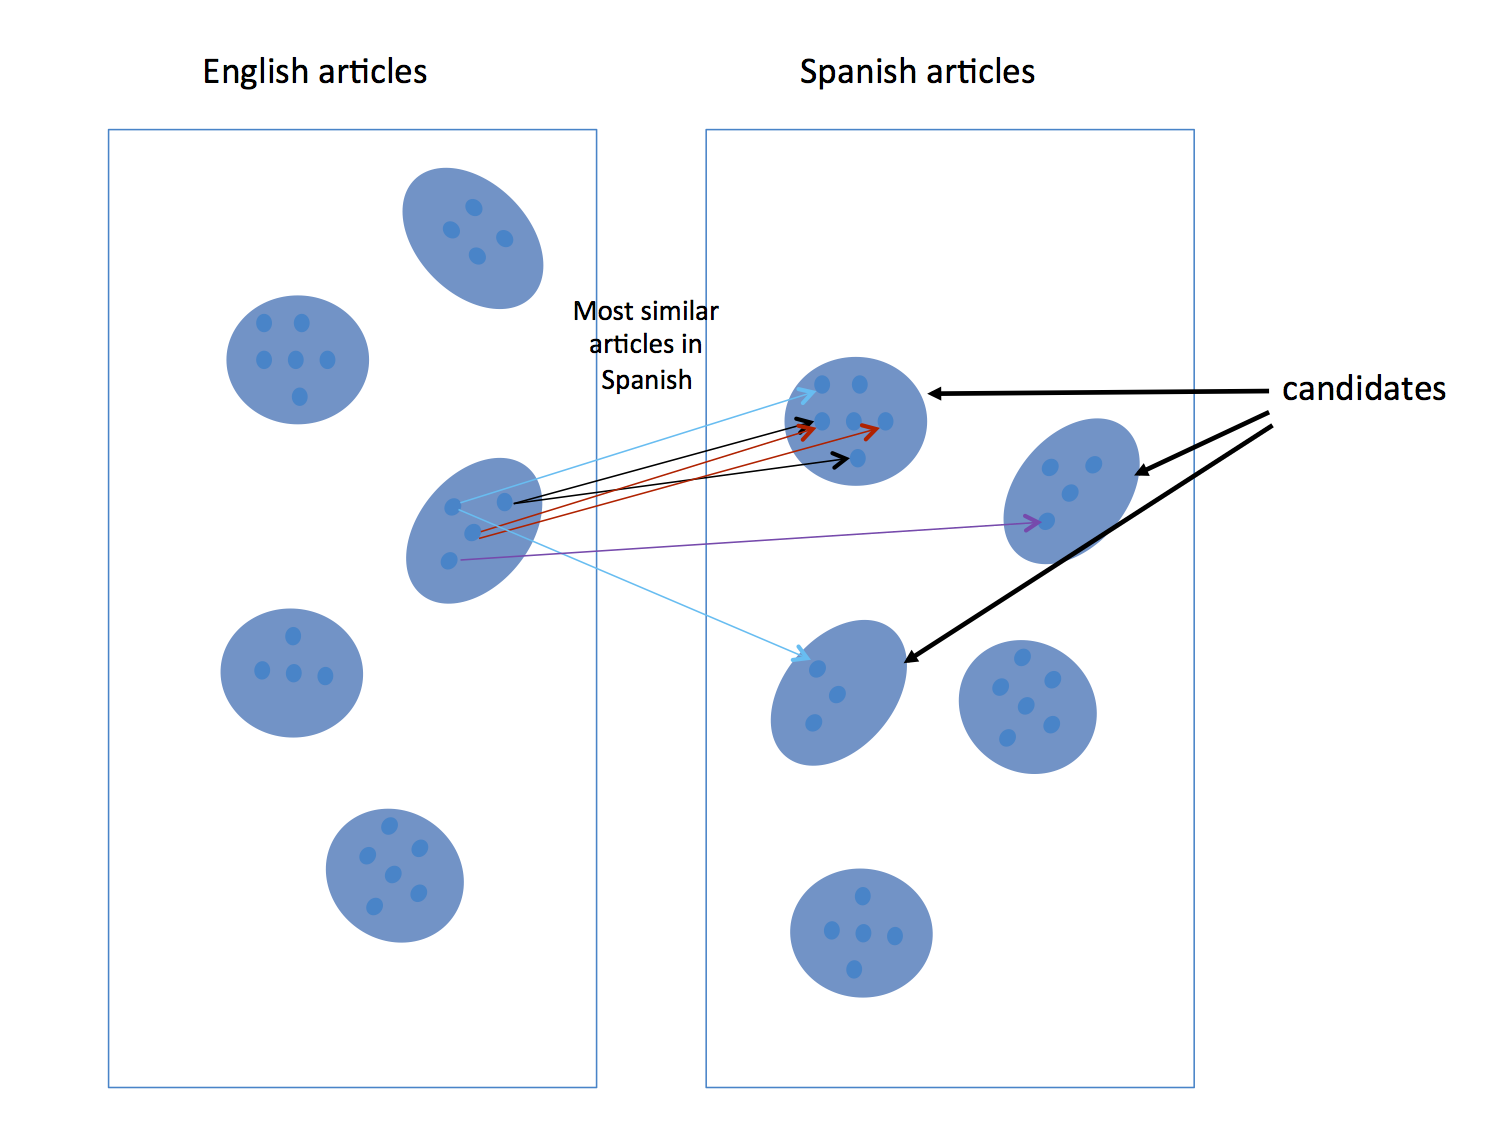
\includegraphics[width=0.6\textwidth]{clusters}
\caption{\label{fig:clusters}  Given clusters of articles in different languages, the goal of  linking is to match clusters which have similar content across languages. The challenge in linking is to overcome the errors in the clustering and differing content as well as make the approach scalable. Therefore, we first identify candidate clusters. }
\end{figure}

Furthermore, the matching of clusters is a \emph{generalized matching}. We cannot assume that there is only one cluster per language per event, nor can we assume complete coverage -- that there exists at least one cluster per event in every language. This implies that we cannot make any assumptions on the matching, e.g. one-to-one, complete, etc. This excludes the use of standard weighted bipartite matching type of algortihms for this problem. An example is shown in Figure~\ref{fig:clusters}, where a cluster may contain articles which are closely matched with many clusters in a different language.



We impose an additional requirement.  Identification of the equivalent clusters cannot be done exhaustively -- for a cluster $c_i$ we wish to avoid testing all other clusters for all the other languages. Performing exhaustive comparison for each cluster $c_i$ would result in $O(N^2)$ tests, where $N$ is the number of all clusters (over all languages), which is not feasible when the number of clusters is on the order of tens of thousands.

\begin{comment}
One of the use cases where article linking information can be applied is also in an online system for detection of world events, called Event Registry\cite{}. Event Registry is a repository of events, where events are automatically identified by analyzing news articles. The term event is vague and ambiguous, but for the practical purposes we define it as ``any significant happening that is being reported about in the media''.

Event Registry works by collecting and analyzing news articles that are published by news outlets in different languages all over the world. Collected articles are first semantically annotated by identifying in them mentions of relevant concepts -- either entities or important keywords. The disambiguated and entity linking of the concepts is done using Wikipedia as the main knowledge base. The key step in Event Registry is then to apply an online clustering algorithm on the articles in order to identify groups of articles that are discussing the same event. For each new article, the clustering algorithm determines if the article should be assigned to some existing cluster or into a new cluster. The underlying assumption is that articles that are describing the same event are similar enough and will therefore be put into the same cluster.

In short, the article clustering works as follows (details are available in \cite{Brank2014}). First we create a new document by joining the title and the body of the article. We then tokenize the document, remove the stop words and stem the words. The remaining words are represented as a vector in the vector-space model. Each value in the vector is additionally normalized using TF-IDF. After normalization, we use the vector to find the most similar existing cluster. To be able to compare the vector with a cluster we first need a vector representation for each of the clusters. This is done by computing a centroid vector of the cluster by simply averaging the vectors of the articles in the cluster. By computing the cosine similarity of the article vector with each of the centroid vectors we then find the cluster with the highest similarity. If the highest similarity is above the selected threshold (we used 0.4 in our experiments), the article is assigned to the corresponding cluster, otherwise a new cluster is created, initially containing only the single article.

Since articles about an event are commonly written only for a short period of time, we remove clusters once the oldest article in the cluster becomes more than 4 days old. This housekeeping mechanism prevents the clustering from becoming slow and also ensures that articles are not assigned to obsolete clusters.

In order to treat the cluster as describing an event in Event Registry, the cluster has to grow above a certain number of articles (the number depends on the language). This condition ensures that only content that receives a sufficient coverage in the media is treated as an event. Once a new event is identified, a new unique ID is assigned to it and the main information about the event is then automatically extracted by analyzing the articles assigned to it. The extracted information includes properties such as the date of the event, the location, who is involved in it, what the event is about, etc.

The clustering of articles is done for each language separately -- English articles are, for example, clustered separately from Spanish articles. When events are identified, they will therefore be identified from clusters in each language separately. As a result, the same event will be represented in Event Registry with two or more event IDs, and each event will only contain coverage in a single language. To avoid this problem we want to exploit the available information about the similarity of the articles in a cluster with articles in other languages. Using this information we hope to be able to connect clusters in different languages and represent them using a single event ID.

\subsection{Problem definition}

The problem in the second phase of the pipeline is to identify the clusters (given?) describing the same events. Each article $a_i$ is written in a language $l$, where $l \in L = \{l_1,l_2,...,l_k\}$. For each language $l$, we generate and maintain a set of language-specific clusters $C_l$. That is, all articles are in language $l$. For any cluster $c_i \in C_{l_a}$, we would like to identify clusters $c_j \in C_{l_b}$ (where $l_a \neq l_b$) that describe the same event as $c_i$. We define \emph{equivalent clusters} as  pairs $(c_i,c_j)$ such that both clusters in the pair describe the same event in languages $C_{l_a}$ and $C_{l_b}$ respectively.


\end{comment}

\subsection{Related work}

Although there are a number of services that aggregate news by identifying clusters of similar articles, there are almost no services that provide linking of clusters over different languages. Google News as well as Yahoo! News are able to identify clusters of articles about same event, but they offer no linking of clusters across languages. The only service that we found, which provides cross-lingual cluster linking, is the European Media Monitor (EMM)~\cite{Steinberger2008}. EMM clusters articles in 60 languages and then tries to determine which clusters of articles in different languages describe the same event. To achieve cluster linking, EMM uses three different language independent vector representations for each cluster. First vector contains the weighted list of references to countries mentioned in the articles, while the second vector contains the weighted list of mentioned people and organizations. The last vector contains the weighted list of Eurovoc subject domain descriptors. These descriptors are topics, such as \emph{air transport}, \emph{EC agreement}, \emph{competition} and \emph{pollution control} into which articles are automatically categorized~\shortcite{Pouliquen2006}. Similarity between clusters is then computed using a linear combination of the cosine similarities computed on the lists. If the similarity is above the threshold, the clusters are linked.

A system that is significantly different, but worth mentioning is the GDELT project~\cite{Leetaru2013Gdelt}. In GDELT, events are also extracted from articles, but in their case, an event is specified in a form of a triple containing two actors and a relation. The project contains an extensive vocabulary of possible relations, mostly related to political events. In order to identify events, GDELT collects articles in more than 65 languages and uses machine translation to translate them to English. All information extraction is then done on the translated article.

\subsection{Algorithm}

In order to identify clusters $c_j$ that are equivalent to cluster $c_i$, we have developed a two-stage algoirhtm. For a cluster $c_i$, we first efficiently identify a small set of candidate clusters and then find those clusters among the candidates, which are equivalent to $c_i$. An example is  shown in  Figure~\ref{fig:clusters}.

The details of the first step are described in Algorithm~\ref{cluster_merge_algo1}. The algorithm begins by individually inspecting each article $a_i$ in the cluster $c_i$. Using a chosen method for computing cross-lingual document similarity (see Section~\ref{sec:models}), it identifies the 10 most similar articles to $a_i$ in each language $l \in L$. For each  similar article $a_j$, we identify its corresponding  cluster $c_j$ and add it to the set of candidates. The set of candidate clusters obtained in this way is several orders of magnitude smaller than the number of all clusters. Although computed document similarities are approximate, our  assumption  is that articles in different languages describing the same event, will generally have a higher similarity than articles about different events. While this assumption does not always hold, redundancy in the data mitigates these false positives. Since we compute the 10 most similar articles for each article in $c_i$, we are likely to identify all the relevant candidates for cluster $c_i$.

\begin{algorithm}[t!]
\SetKwInput{KwInput}{input}\SetKwInput{KwOutput}{output}
\KwInput{test cluster $c_i$,\\a set of clusters $C_l$ for each language $l \in L$}
\KwOutput{a set of clusters $C$ that are potentially equivalent to $c_i$}
$C = \{\}$\;
\For{article $a_i \in c_i$} {
    \For{language $l \in L$} {
        \tcc{use CCA to find 10 most similar articles to article $a_i$ in language $l$}
        $SimArt = getCCASimArts(a_i, l)$\;
        \For{article $a_j \in SimArt$} {
            \tcc{find cluster $c_j$ to which article $a_j$ is assigned to}
            $c_j := c ; c \in C_l, a_j \in c$\;
            \tcc{add cluster $c_j$ to the set of candidates $C$}
            $C \leftarrow c_j$\;
        }
    }
}
\caption{Algorithm for identifying candidate clusters $C$ that are potentially equivalent to $c_i$}
\label{cluster_merge_algo1}
\end{algorithm}

The second stage of the algorithm (described in the Algorithm~\ref{cluster_merge_algo2}.) determines which (if any) of the candidate clusters are equivalent to $c_i$. We approach this as a supervised learning problem. For each candidate cluster $c_j \in C'$, we compute a vector of learning features that should be indicative of whether the $c_i$ and $c_j$ are equivalent or not. The details of our chosen features will be described in the following Section. Once these features are computed, we apply a classification model which was trained using a  dataset  of hand-labeled examples. If the model predicts that tested clusters are equivalent, the $c_j$ is added to the set $C'$.

\begin{algorithm}[tb!]
\SetKwInput{KwInput}{input}\SetKwInput{KwOutput}{output}
\KwInput{test cluster $c_i$,\\
a set of candidate clusters $C$ that are potentially equivalent to $c_i$\\
classification model $M$ trained on the hand-labeled examples}
\KwOutput{a set of clusters $C'$ that are equivalent to $c_i$}

$C' = \{\}$\;
\For{cluster $c_j \in C$} {
    \tcc{extract a vector of features for cluster pair $c_i$ and $c_j$}
    $\vec{v} = f(c_i, c_j)$\;
    \tcc{classify the feature vector $\vec{v}$ using the model $M$}
    $pred = M(\vec{v})$\;
    \If{$pred$ = true} {
        $C' \leftarrow c_j$
    }
}
\caption{Algorithm for identifying clusters $C'$ that are equivalent to cluster $c_i$}
\label{cluster_merge_algo2}
\end{algorithm}

\subsection{Training a classification model}

In order to train a classification model for predicting whether two clusters are equivalent, we must first have labeled data. To obtain the data, we used two human annotators. The annotators were provided with an interface displaying information about the articles in two clusters and their task was to determine if the clusters were equivalent or not. To obtain a pair of clusters $(c_i, c_j)$ to annotate, we first randomly chose a cluster $c_i$, used the Algorithm~\ref{cluster_merge_algo1} to compute a set of potentially equivalent clusters $C$ and randomly chose a cluster $c_j \in C$.

The dataset provided by the annotators contains 808 examples, of which 402 are equivalent clusters pairs and 406 are not. Clusters in each learning example are either in English, Spanish or German. Although Event Registry imports articles in other languages as well, we restricted our experiments to these three languages, since they have the highest volume of articles which makes the training problem similarly hard \todo{doesnt this make it easier?}.

To build a classification model we first extract  informative features from the labeled examples. Based on the availability of the data, we extracted the following groups of features:

\begin{itemize}
\item {\bf Cross-lingual article linking features}. Cross-lingual article linking information was already used to obtain candidates for the equivalent clusters. Additionally, it can also be used to provide valuable  features for learning. There are two main features that we extract from article links between clusters -- \texttt{linkCount} and \texttt{avgSimScore}. \texttt{linkCount} is the number of times an article $a_i \in c_i$ has as one of the 10 most similar articles an article $a_j \in c_j$. In other words, it is the number of times an article from $c_i$ has a very similar article, which is in $c_j$. Beside the number of links between the two clusters we can also take into account the similarity scores of the links. The \texttt{avgSimScore} is the feature that represents the average similarity score of the links between the two clusters.

\item {\bf Concept related features}. As mentioned before, articles that are imported into Event Registry are first semantically annotated by linking mentioned entities and keywords to the corresponding Wikipedia pages. Whenever Barack Obama is, for example, mentioned in the article, the article is annotated with a link to his Wikipedia page (\emph{http://en.wikipedia.org/wiki/Barack\_Obama}). In the same way all mentions of people, locations, organizations and even ordinary keywords (e.g. bank, tax, ebola, plane, company) are annotated. Although the Spanish article about Obama will be annotated with his Spanish version of the Wikipedia page, in many cases we can link the Wikipedia pages to their English versions. This can be done since Wikipedia itself provides information regarding which pages in different languages represent the same concept/entity. Using this approach, the word ``avi\'on'' in a Spanish article will be annotated with the same concept as the word ``plane'' in an English article. Although the articles are in different languages, the annotations can therefore provide a shared vocabulary that can be used to compare articles/clusters. By analyzing all the articles in clusters $c_i$ and $c_j$, we can identify the most relevant entities and keywords for each cluster. Additionally, we can also assign weights to the concepts based on how frequently they occur in the articles in the cluster. From the list of relevant concepts and corresponding weights, we consider the following features: \texttt{entityCosSim} which represents the cosine similarity on the vector of entities mentioned in both clusters; \texttt{keywordCosSim} which represents the cosine similarity on the keywords only; for cases where the weights are not relevant, we have also added two additional features - (\texttt{entityJaccardSim} and \texttt{keywordJaccardSim}), where Jaccard similarity is used instead of the cosine similarity.

\item {\bf Miscellaneous features}. This group contains three miscellaneous features that seem discriminative but are unrelated to the previous two groups. The first feature is related to the event location. By considering the locations mentioned in the articles in a cluster, we are able to estimate where an event occurred. The \texttt{hasSameLocation} feature is a boolean variable that is true when the location of the event in both clusters is the same. Another important feature is related to the time when the articles in the clusters were published. For each cluster, we first compute the average publication time and date of the articles. The \texttt{timeDiff} is then defined as the absolute difference in hours between the two computed dates. The final feature we consider is computed by analyzing the mentions of dates in the articles. Using an extensive set of regular expressions, we are able to detect mentions of dates in different forms. To compute the feature \texttt{sharedDates} we start by identifying the list of dates mentioned in articles in each cluster separately. The value of \texttt{sharedDates} is then determined as the ratio of all dates that are detected in both clusters.\todo{this should be made more explicit/}

\end{itemize}

Using the  features described above and the user-provided labels, we train a classification model $M$ which is used in Algorithm~\ref{cluster_merge_algo2} to classify a new cluster pair as equivalent or not. The classification algorithm that we used to train a model was a linear SVM method.




\section{Evaluation}

We describe the datasets involved in the experiments and two evaluations: comparing the crosslingual approaches on an information retrieval task, and evaluation of cross-lingual event linking.

\subsection{Datasets}
%\emph{Andrej started shuffling it, will do it till Monday :) }
%{\oldText{Taken from ITI paper}
To investigate the empirical performance of the low rank approximations we will test the algorithms on a large-scale, real-world multilingual dataset that we extracted from Wikipedia by using inter-language links as an alignment. This  results in a large number of weakly comparable documents in more than $200$ languages. Wikipedia is a large source of multilingual data that is especially important for the languages for which no translation tools, multilingual dictionaries as Eurovoc, or strongly aligned multilingual corpora as Europarl are available. Documents in different languages are related with so called 'inter-language' links that can be found on the left of the Wikipedia page. The Wikipedia is constantly growing. There are currently 12 Wikipedias with more than $10^6$ articles, $52$ with more than $10^5$ articles, $129$ with more than $10^4$ articles, and $236$ with more than $1000$ articles.
%Wikipedia uses special user-friendly markup language that is very easy to write but very hard to parse. Simplicity of language can cause ambiguities and moreover it is constantly changing. For example, separator | can be used in %different contexts.

%Wikipedia raw xml dumps of all currently $288$ active editions were downloaded from the Wikipedia dump page\href{http://dumps.wikimedia.org}. The xml files are too large to be parsed with DOM like parser that needs to store the whole xml tree in the memory, instead we implemented Sax like parser that tries to simulate behavior of Wikipedia official parser and is as simple, fast and error prone as possible. We parse all Wikipedia markup but do not expand the templates.
Each Wikipedia page is embedded in the page tag. First we check if the title of the page consists of any special namespace and do not process such pages. Then we check if this is a redirection page and we store the redirect link as inter-language links can point to redirection link also. If nothing of the above applies we extract the text and parse the Wikipedia markup. Currently all the markup is removed.

We get inter-language link matrix using previously stored redirection links and inter-language links. If inter-language link points to the redirection we replace it with the redirection target link. It turns out that we obtain the matrix $M$ that is not symmetric, consequently the underlying graph is not symmetric. That means that existence of the inter-language link in one way (i.e. English to German) does not guarantee that there is an inter-language link in the reverse direction (German to English). To correct this we transform this matrix to symmetric by computing $M+M^T$ and obtaining an undirected graph. In the rare case that we have multiple links pointing from the document, we pick the first one that we encountered. This matrix enables us to build an alignment across all Wikipedia languages.
%}

\subsection{Wikipedia Information Retrieval}

Mate retrieval results

\subsection{Experiments With Missing Alignment Data}
%\emph{Andrej started working on this, done by Monday}
%{\oldText{Taken from XLite paper}
%To investigate the empirical performance of our algorithm we will test it on a large-scale, real-world multilingual dataset that we extracted from Wikipedia  by  using so called 'inter-language' links as an alignment.
 In this subsection we will investigate the empirical performance of cca hub approach. We will demonstrate that this approach can be successfully applied even in the case of missing alignment information.
 To this purpose we select a subset of Wikipedia languages containing three major languages, English--\emph{en} (hub language), Spanish--\emph{es}, Russian--\emph{ru}, and five minority (in the sense of Wikipedia sizes) languages, Slovenian--\emph{sl}, Piedmontese--\emph{pms}, Waray-Waray--\emph{war} (all with about 2 million native speakers), Creole--\emph{ht} (8 million native speakers), and Hindi--\emph{hi} (180 million native speakers). For preprocessing we remove the documents that contain less than 20 different words (stubs) and remove words occurring in less than 50 documents as well as the top 100 most frequent words (in each language separately). We represent the documents as normalized TFIDF\cite{Salton88term-weightingapproaches} weighted vectors.
 %These are languages with Wikipedia article sizes comparable to the minority languages.  (since the number of speakers does not directly correlate with the number of Wikipedia articles). The prime hub candidate is the English %language which is well aligned with all other Wikipedia languages, although the alignment quality varies quite a bit. Furthermore, we remove the documents that contain less than 20 different words and remove words that are too %infrequent as well as the top 100 most frequent words in the vocabularies.
 Although the English language is well aligned with all Wikipedia languages, we must note that quality of alignment varies quite a bit, especially in the case of small Wikipedias.
 Furthermore, we call the document consisting of less than 20 different words, a stub. This documents are typically garbage, the titles of the columns in the table, remains of the parsing process, or Wikipedia articles with very little or no information contained in one or two sentences.


The evaluation is based on splitting the data into training and test sets (described later). On the training set, we perform the two step procedure to obtain the common document representation as a set of mappings $P_i$. A test set for each language pair, $test_{i,j} = \{(x_\ell,y_\ell) | \ell = 1:n(i,j)\} $, consists of comparable document pairs (linked Wikipedia pages), where $n(i,j)$ is the test set size. We evaluate the representation by measuring mate retrieval quality on the test sets: for each $\ell$, we rank the projected documents $P_j(y_1),\ldots, P_j(y_{n(i,j)})$ according to their similarity with $P_i(x_\ell)$ and compute the rank of the mate document $r(\ell) = rank(P_j(y_\ell))$. The final retrieval score (between -100 and 100) is computed as: $\frac{100}{n(i,j)} \cdot \sum_{\ell = 1}^{n(i,j)} \left( \frac{n(i,j) - r(\ell)}{n(i,j) -1} -0.5\right)$. A score that is less than 0 means that the method performs worse than random retrieval and a score of 100 indicates perfect mate retrieval. The mate retrieval results are included in Table \ref{table:retrieval}.

We observe that the method performs well on all pairs between languages: \emph{en}, \emph{es}, \emph{ru}, \emph{sl}, where at least 50,000 training documents are available. We notice that taking $k = 500$ or $k = 1000$ multilingual topics usually results in similar performance, with some notable exceptions: in the case of (\emph{ht}, \emph{war}) the additional topics result in an increase in performance, as opposed to (\emph{ht},\emph{pms}) where performance drops, which suggests overfitting. The languages where the method performs poorly are \emph{ht} and \emph{war}, which can be explained by the quality of data (see Table \ref{table:rank} and explanation that follows). In case of \emph{pms}, we demonstrate that solid performance can be achieved for language pairs (\emph{pms}, \emph{sl}) and (\emph{pms}, \emph{hi}), where only 2000 training documents are shared between \emph{pms} and \emph{sl} and no training documents are available between \emph{pms} and \emph{hi}. Also observe that in the case of (\emph{pms}, \emph{ht}) the method still obtains a score of 62, even though training set intersection is zero and \emph{ht} data is corrupted, which we will show in the next paragraph.
{
\renewcommand\tabcolsep{3pt}
\begin{table}[h!]
\caption{Pairwise retrieval, 500 topics;1000 topics}\label{table:retrieval}
\begin{center}
\begin{tabular}{|c|c|c|c|c|c|c|c|c|}
\cline{1-9}
&	en&	es&	ru&	sl&	hi&	war&	ht&	pms\\\cline{1-9}
en&	    &	98~-~98&	95~-~97&	97~-~98&	82~-~84&	76~-~74&	53~-~55&	 96~-~97\\
\cline{1-9}
es&	97~-~98&	&	94~-~96&	97~-~98&	85~-~84&	76~-~77&	56~-~57&	96~-~96\\
\cline{1-9}
ru&	96~-~97&	94~-~95&	&	97~-~97&	81~-~82&	73~-~74&	55~-~56&	96~-~96\\
\cline{1-9}
sl&	96~-~97&	95~-~95&	95~-~95&	&	91~-~91&	68~-~68&	59~-~69&	93~-~93\\
\cline{1-9}
hi&	81~-~82&	82~-~81&	80~-~80&	91~-~91&	&	68~-~67&	50~-~55&	87~-~86\\
\cline{1-9}
war&	68~-~63&	71~-~68&	72~-~71&	68~-~68&	66~-~62&	&	28~-~48&	 24~-~21\\
\cline{1-9}
ht&	52~-~58&	63~-~66&	66~-~62&	61~-~71&	44~-~55&	16~-~50&	&	62~-~49\\
\cline{1-9}
pms&	95~-~96&	96~-~96&	94~-~94&	93~-~93&	85~-~85&	23~-~26&	66~-~54&	 \\
\cline{1-9}
\end{tabular}
\end{center}
\end{table}
}

We now describe the selection of train and test sets. We select the test set documents as all multi-lingual documents with at least one nonempty alignment from the list: (\emph{hi}, \emph{ht}), (\emph{hi}, \emph{pms}), (\emph{war}, \emph{ht}), (\emph{war}, \emph{pms}). This guarantees that we cover all the languages. Moreover this test set is suitable for testing the retrieval thorough the hub as the chosen pairs have empty alignments. The remaining documents are used for training. In Table \ref{table:train_test}, we display the corresponding sizes of training and test documents for each language pair. The first row represents the size of the training sets used to construct the mappings in low dimensional language independent space using the English--\emph{en} as a hub. The diagonal elements represent number of the unique training documents and test documents in each language.

{
\renewcommand\tabcolsep{3pt}
\begin{table}[h!]
\caption{Pairwise training:test sizes (in thousands)}
\label{table:train_test}
{
\small
\begin{tabular}{c|c|c|c|c|c|c|c|c|}
&	en&	es&	ru&	sl&	hi&	war&	ht&	pms\\\cline{1-9}
en&	671~-~4.64&	463~-~4.29&	369~-~3.19&	50.3~-~2&	14.4~-~2.76&	8.58~-~2.41&	 17~-~2.32&	16.6~-~2.67\\
\cline{2-9}
es&	\multicolumn{1}{c|}{}	&	463~-~4.29&	187~-~2.94&	28.2~-~1.96&	8.72~-~2.48&	 6.88~-~2.4&	13.2~-~2&	 13.8~-~2.58\\
\cline{3-9}
ru&	\multicolumn{2}{c|}{}	&	369~-~3.19&	29.6~-~1.92&	9.16~-~2.68&	2.92~-~1.1&	 3.23~-~2.2&	10.2~-~1.29\\
\cline{4-9}
sl&	\multicolumn{3}{c|}{}	&	50.3~-~2&	3.83~-~1.65&	1.23~-~0.986&	0.949~-~1.23&	 1.85~-~0.988\\
\cline{5-9}
hi&	\multicolumn{4}{c|}{}	&	14.4~-~2.76&	0.579~-~0.76&	0.0~-~2.08&	0.0~-~0.796\\
\cline{6-9}
war&	\multicolumn{5}{c|}{}	&	8.58~-~2.41&	0.043~-~0.534&	0.0~-~1.97\\
\cline{7-9}
ht&	\multicolumn{6}{c|}{}	&	17~-~2.32&	0.0~-~0.355\\
\cline{8-9}
pms&	\multicolumn{7}{c|}{}	&	16.6~-~2.67\\
\cline{9-9}
\end{tabular}
}
\end{table}
}

We further inspect the properties of the training sets by roughly estimating the fraction \texttt{rank(A)/min(size(A))} for each training English matrix and its corresponding mate matrix. Ideally, these two fractions are approximately the same so  both aligned spaces should have reasonably similar dimensionality. We display these numbers as pairs in Table \ref{table:rank}.

\begin{table}[h]
\caption{Dimensionality drift}
\label{table:rank}
\begin{tabular}{|c|c|c|c|c|c|c|}
\cline{1-7}
(en, de)     &   (en, ru)     &   (en, sl)       &     (en, hi)&   (en, war)      &      (en, ht) &   (en, pms)\\
\cline{1-7}
(0.81, 0.89)   &  (0.8, 0.89)  &   (0.98, 0.96)    &    (1, 1)  &   (0.74, 0.56)  &      (1, 0.22)  &   (0.89, 0.38)\\
\cline{1-7}
\end{tabular}
\end{table}

It is clear that in the case of Creole language only at most $22\%$ documents are unique and suitable for the training. Though we removed the stub documents, many of remaining documents are almost the same, as the quality of some minor Wikipedias is low. This was confirmed for Creole, Waray-Waray, and Piedmontese language by manual inspection. The low quality documents correspond to templates about the year, person, town, etc. and contain very few unique words.

We also have a problem with the quality of the test data. For example, if we look at test pair (\emph{war}, \emph{ht}) only 386/534 Waray-Waray test documents are unique but on other side almost all Creole test documents (523/534) are unique. This indicates a poor alignment which leads to poor performance.
%}

\subsection{Evaluation Of Cross-Lingual Event Linking}

In order to determine how accurately we can predict cluster equivalence we have performed two experiments. In the first experiment we wanted to test how well do the individual approaches for cross-lingual article linking perform when used for linking the clusters about the same event. In the second experiment we tested how accurate is the prediction model when trained on different subsets of learning features. To evaluate the prediction accuracy for a given dataset we used 10-fold cross validation. In this technique, the dataset is partitioned into 10 folds, where 9 folds are used for training a model and the left-out fold is then used to test the accuracy of the model. The learning and testing process is repeated 10 times, each time with a different left-out fold.

In Section~\ref{sec:models} we have described three main algorithms for identifying similar articles in different languages. These algorithms were $k$-means, LSI and CCA. To test which of these algorithms performs best we performed the following test. Using each algorithm, we analyzed all articles in Event Registry to find the most similar articles in other languages. The values of the cross-lingual article linking features (\texttt{linkCount} and \texttt{avgSimScore}) were then recomputed for all annotated learning examples. A dataset with only these two features and the label was constructed and used to test how accurate prediction models can be induced using the data. The results of the experiment are shown in Table~\ref{table:linkingEvalAlgos}. The table shows for each of the algorithms the obtained classification accuracy, precision and recall. We can see that the most informative features for cluster linking are obtained using the CCA algorithm, while $k$-means performs the worse. Firstly we verified the AMRR (average of mean reciprocal ranks over all language pairs) performance of approaches by holding out $15000$ aligned test documents and using $300000$ aligned documents
 as the training set. Figure~\ref{pc:AMRR} shows AMRR score as the function of the number of feature vectors. It is clear that CCA outperforms LSI approach and K-means lags far behind.
Furthermore we inspected how number of features influences the accuracy of cluster linking. As we can see from Table~\ref{table:linkingEvalAlgos} choosing number of features vectors larger than $500$ barely effects linking performance. That is probably due to overfitting. Moreover we tested the performance of detecting large/small cluster linking, see Table~\ref{table:linkingEvalAlgosLargeSmall}.  As expected we obtained that it is harder to link small clusters and we need better retrieval. Hub CCA outperforms other methods in this sense also, probably as it has the best retrieval performance, see Figure~\ref{pic:AMRR}.

%{\oldText{TODO:} add some explanation why this might be so.}
%\emph{Andrej adds some tests, new experiment description graphs, and explanations for performance, done by Monday}
%15000 test documents, around 300 000 sth training documents
%Results for feature spaces of dimensions 500, 800, 1000  overfitting, 800 minor improvement
%Timex complexity of similarity computation scales linearly with dimension space. We double numbers of articles and decrease memory requirements by 1/2.
%CCA       CA          AUC         Prec        Recall
%CCA =     [0.7882      0.8504      0.7692	   0.8209
%           0.7957      0.8624      0.7788      0.8234
%           0.8031      0.8654      0.8015      0.8035];
%LSIS=     [0.7994      0.8627      0.7778      0.8358
%           0.7956      0.8634      0.7828      0.8159
%           0.7994      0.8642      0.8030      0.7910];
%LSIW=     [0.7894      0.8606      0.7673      0.8284;
%           0.7870      0.8632      0.7662      0.8234;
%           0.8018      0.8663      0.7854      0.8284];

%AMPR as function of the number of feature vectors
%500 is good, 800 better, 1000 overfitting, noise!
\begin{figure}
\caption{Average of mean reciprocal ranks}
\label{pic:AMRR}
%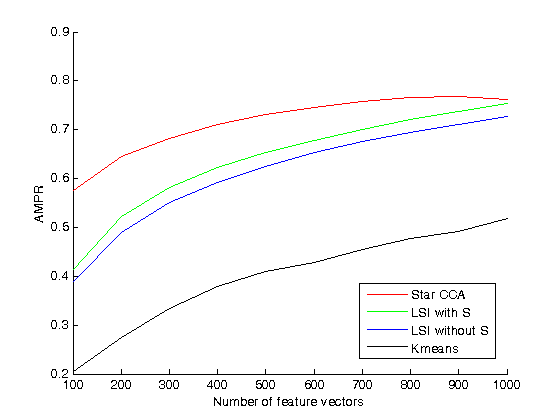
\includegraphics{slika.png}
% This file was created by matlab2tikz.
% Minimal pgfplots version: 1.3
%
%The latest updates can be retrieved from
%  http://www.mathworks.com/matlabcentral/fileexchange/22022-matlab2tikz
%where you can also make suggestions and rate matlab2tikz.
%
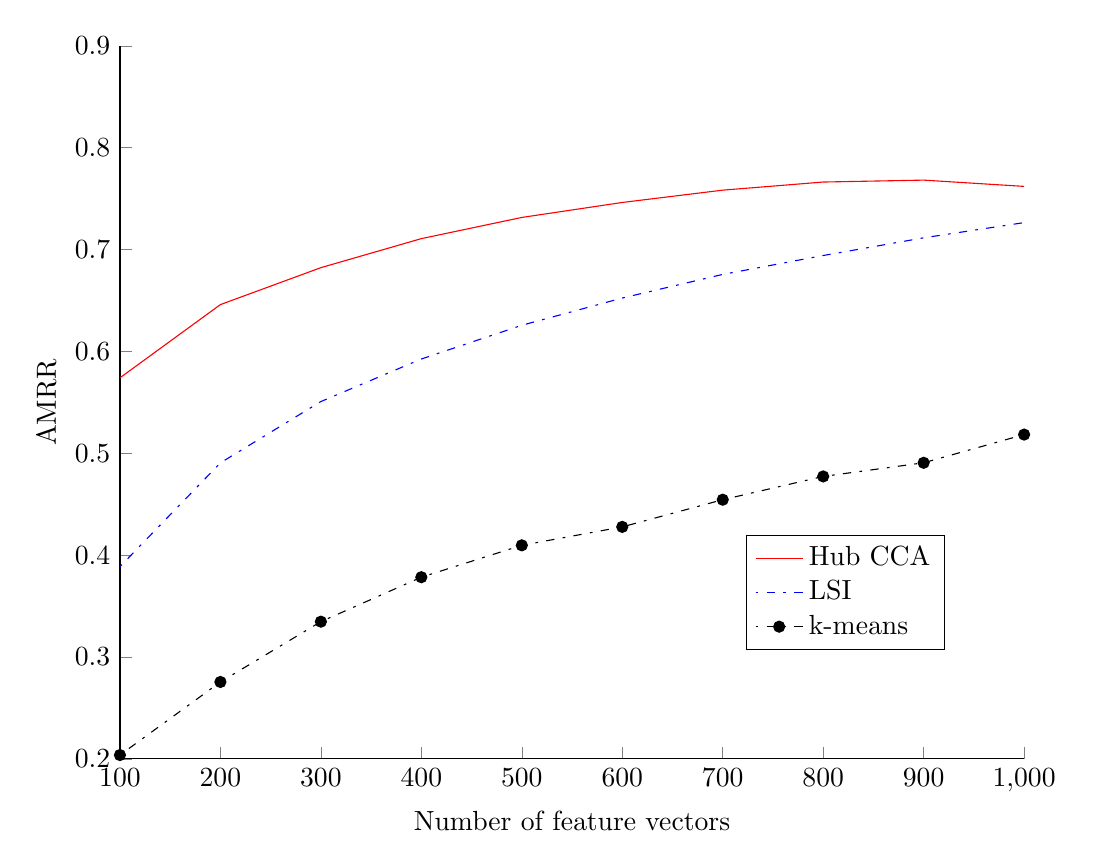
\begin{tikzpicture}

\begin{axis}[%
width=4.520833in,
height=3.565625in,
at={(0.758333in,0.48125in)},
scale only axis,
every outer x axis line/.append style={black},
every x tick label/.append style={font=\color{black}},
xmin=100,
xmax=1000,
xlabel={Number of feature vectors},
every outer y axis line/.append style={black},
every y tick label/.append style={font=\color{black}},
ymin=0.2,
ymax=0.9,
ylabel={AMRR},
axis x line*=bottom,
axis y line*=left,
legend style={at={(0.692559,0.152778)},anchor=south west,legend cell align=left,align=left,draw=black}
]
\addplot [color=red,solid]
  table[row sep=crcr]{%
100	0.574094231082746\\
200	0.645978450670063\\
300	0.682226506762222\\
400	0.710722094692085\\
500	0.731517169423203\\
600	0.746223870375363\\
700	0.758312886611436\\
800	0.766279310559898\\
900	0.768159613081689\\
1000	0.76200517888255\\
};
\addlegendentry{Hub CCA};

\addplot [color=blue,dash pattern=on 1pt off 3pt on 3pt off 3pt]
  table[row sep=crcr]{%
100	0.388773162433835\\
200	0.49061571487968\\
300	0.550801867794634\\
400	0.592565604079171\\
500	0.625657099289601\\
600	0.65240747960386\\
700	0.675602522126668\\
800	0.694149727717174\\
900	0.711511053167843\\
1000	0.726455461653153\\
};
\addlegendentry{LSI};

\addplot [color=black,dash pattern=on 1pt off 3pt on 3pt off 3pt,mark=*,mark options={solid}]
  table[row sep=crcr]{%
100	0.203799120889507\\
200	0.275537657758881\\
300	0.334738107118325\\
400	0.378380649062479\\
500	0.409668545430712\\
600	0.427765004442194\\
700	0.454449272479224\\
800	0.477291178317808\\
900	0.490692600634559\\
1000	0.518392823243787\\
};
\addlegendentry{k-means};

\end{axis}
\end{tikzpicture}%
\end{figure}
%Why the hub approach?
%Optimize for language pairs in the system that have the largest number of articles in the system!
%Is star CCA really the best???
%Maybe omit this table?
\begin{table}[h]
\caption{Accuracy of cluster linking with 500 - 800 - 1000 features obtained from different cross-lingual similarity algorithms}
\label{table:linkingEvalAlgos}
\begin{center}
\begin{tabular}{|c|c|c|c|}
  \hline
  \cline{1-4}
  Models & CA & Precision & Recall \\ \cline{1-4}
  CCA      & 78.2 - 79.6 - 80.3 \% & 76.3 - 78.0 - 80.5 \%  & 81.6 - 82.1 - 79.9 \%  \\ \cline{1-4}
  LSI      & 78.9 - 78.7 - 80.6 \%  & 76.8 - 77.0 - 78.7 \%  & 83.3 - 80.6 - 83.6 \%  \\ \cline{1-4}
 $k$-means & 73.9\phantom{ - 78.7 - 80.6 }\% & 69.5\phantom{ - 78.7 - 80.6 }\%  & 84.6\phantom{ - 78.7 - 80.6 }\%  \\ \cline{1-4}
\end{tabular}
\end{center}
\end{table}

\begin{table}[h]
\caption{Accuracy of large/small cluster linking with $500$ features obtained from different cross-lingual similarity algorithms}
\label{table:linkingEvalAlgosLargeSmall}
\begin{center}
\begin{tabular}{|c|c|c|c|}
  \hline
  \cline{1-4}
  Models & CA & Precision & Recall \\ \cline{1-4}
  CCA      & 81.2 - 77.8 \% & 80.5 - 74.5 \%  & 91.3 - 57.5 \%  \\ \cline{1-4}
  LSI      & 82.8 - 76.4 \% & 81.3 - 70.9 \%  & 93.1 - 57.5 \%  \\ \cline{1-4}
 $k$-means & 75.5 - 71.2 \% & 72.8 - 70.8 \%  & 95.3 - 36.2 \%  \\ \cline{1-4}
\end{tabular}
\end{center}
\end{table}



In the second experiment we wanted to evaluate how relevant individual groups of features are to correctly determine cluster equivalence. For this purpose we tested the accuracies obtained using individual groups of features, as well as using different combination of groups. Since we found the CCA to perform best of the three algorithms, we recomputed $500$ feature vectors with better accuracy and used it to compute the values of the cross-lingual article linking features. Results of the evaluation are shown in Table~\ref{table:linkingEval}. We can see that using a single group of features, the highest prediction accuracy can be achieved using the concept related features. The classification accuracy in this case is 88.8\%. By additionally including also the cross-lingual article linking features, the classification accuracy rises slightly to 89.2\%. Using all three groups of features, the achieved accuracy is 89.6\%.
Based on the results we can make the following conclusions. The cross-lingual similarity algorithms provide valuable information that can be used to identify clusters that describe the same event in different languages. The computed features are however significantly less informative compared to the features computed on the annotated concepts. Nevertheless, the cross-lingual article similarity features are very important for two reasons. The first reason is that they allow us to identify for a given cluster a limited set of candidate clusters that are potentially equivalent. This is a very important feature since it reduces the search space for several orders of magnitude. The second reason for the importance of these features is that concept annotations are not available for all articles. Annotation of news articles is computationally intensive and can only be done for a subset of collected articles.

%\begin{table}[h]
%\caption{Accuracy of cluster linking with features obtained from different cross-lingual similarity algorithms}
%\label{table:linkingEvalAlgos}
%\begin{center}
%\begin{tabular}{|c|c|c|c|}
%  \hline
%  \cline{1-4}
%  Models & CA & Precision & Recall \\ \cline{1-4}
%  CCA & 77.6\% & 78.3 \%  & 81.1\%  \\ \cline{1-4}
%  $k$-means & 73.9\% & 69.5\%  & 84.6\%  \\ \cline{1-4}
%  LSI & 79.2\% & 78.9\%  & 80.6\%  \\ \cline{1-4}
%  \hline
%\end{tabular}
%\end{center}
%\end{table}

\begin{table}[h]
\caption{Accuracy of story linking with different sets of features}
\label{table:linkingEval}
\begin{center}
\begin{tabular}{|c|c|c|c|}
  \hline
  \cline{1-4}
  Features & CA & Precision & Recall \\ \cline{1-4}
  CCA & 77.6\% & 0.783 & 0.811 \\ \cline{1-4}
  Concepts & 88.8\% & 0.884 & 0.891 \\ \cline{1-4}
  Misc & 65.3\% & 0.718 & 0.500 \\ \cline{1-4}
  CCA + concepts & 89.2\% & 0.891 & 0.893 \\ \cline{1-4}
  All & 89.6\% & 0.895 & 0.895 \\ \cline{1-4}
  \hline
\end{tabular}
\end{center}
\end{table}


\section{Discussion}


\subsection{Scaling}
\emph{I think that this section should be short.}
100 languages!
%Memory 100 GB per day
%Newsfeed volume 430k articles per day, 210k english, 36k Spanish, 27k German, 17k French, ....
%Number of similarities, 430k similarities every 200ms, currently could handle 1M articles,
%(n \over 2) 500X500 proxy matrices, 300000x500 Projector matrices, 430000x500 data
%Premultiply with proxy matrices, compare blockwise!
One of the main advantages of our approach is that scales really well. It is fast, very robust to quality of training data, easily extendable, simple to implement and with low machine requirements. Ut currently runs on two Intel Xeon E5-2667 v2, 3.30GHz processor machine with 256GB of RAM. That is enough to do similarity computation over 150 languages if needed. It currently uses Wikipedia as freely available knowledge base.

Currently we compute similarities over $24$ languages with tags: eng, spa, deu, zho, ita, fra, rus, swe, nld, tur, jpn, por, ara, fin, ron, kor, hrv, tam, hun, slv, pol, srp, cat, ukr but we support up to $100$ top Wikipedis languages. Our data stream is Newsfeed(http://newsfeed.ijs.si/) that produces $430k$ unique articles per day. Our system currently computes 400k similiarites per 200ms, that means that we compute $16*10^10$ similarities per day. We
store one day buffer for every language, for that we need 1.5GB of memory, we store documents as 500 dimensional vectors. For each article we compute top $10$ most similar ones in every language.
For all linear algebra matrix and vector operations we use high performance numerical libraries as BLAS, OPENBLAS and Intel MKL. This currently allows us to process more than million articles per day.
In our current implementation we use variation of hub approach. Our projector matrices are of size $500\times 300000,$ so every projector takes about $1.1$ GB of RAM. Moreover we need proxy matrices of size $500x500$ for every language pair. That is 0.5 GB for $24$ languages and $9.2$ GB for $100$ languages. All together we need around 135 GB of RAM for the system with 100 languages. Using proxy matrices we can project all the input documents in the common space. That enables us to do blockwise similarity computations and
additional improvement in our system efficiency. Our code can be therefore easily parallelized using matrix multiplication instead of doing more matrix - vector multiplications. This speeds up our code by factor around $4.$ In this way we obtain some caching gains and ability to use vectorization.
Our system is also easily extendable. If we want to add a language we only need to compute a projector matrix and proxy matrices with all other already available languages.

Comment on the caching gains in our implementation.¸¸Add the conclusion if the story.


\acks{The authors wish to thank blah blah blah.}

\vskip 0.2in
\bibliography{jair}
\bibliographystyle{theapa}

\end{document}



